\beginsong{Jerchenkow}[txt={deutsch von peer (Dieter Krolle), 1958}, mel={nach einem ukrainischen Volkslied}, bo={214}, pfii={40}, pfiii={18}, siru={148}, index={Jeden Abend träumt Jerchenkow}]

\beginverse
\endverse
\centering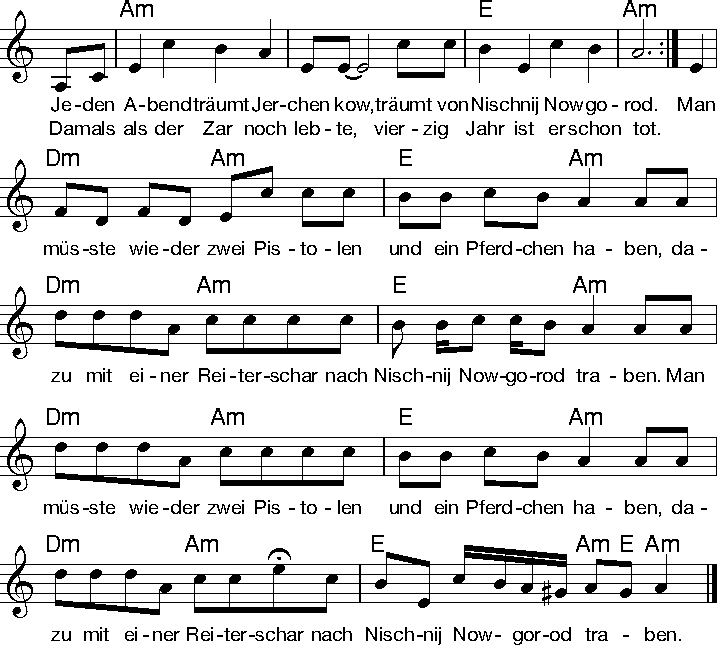
\includegraphics[width=1\textwidth]{Noten/Lied057.pdf}	

\beginverse*
{\nolyrics Zwischenspiel: \[Dm] \[Am] \[E] \[Am] \rep{2} \[E] \[Am]}
\endverse

\beginverse\memorize
Als der \[Am]Mond stand nachts am Himmel, klopften \[E]wir beim Starosten \[Am]an.
Alles klauten wir dem Lümmel, selbst den \[E]roten Sara\[Am]fan.
\endverse

\beginchorus
Man \[Dm]müsste wieder \[Am]zwei Pistolen \[E]und ein Pferdchen \[Am]haben,
da\[Dm]zu mit einer \[Am]Reiterschar nach \[E]Nischnij Nowgorod \[Am]traben.
Man \[Dm]müsste wieder \[Am]zwei Pistolen \[E]und ein Pferdchen \[Am]haben,
da\[Dm]zu mit einer \[Am]Reiterschar nach \[E]Nischnij Nowgorod \[Am]tr\[E]ab\[Am]en.
\lrep \[Dm] \[Am] \[E] \[Am] \rrep  \[E] \[Am]
\endchorus

\beginverse 
Dreimal ^ritt ich nach Odessa, dreimal ^sah ich Peters^burg
als des Zaren Leibkosaken unter ^Hebnio Sara^tow.
\endverse
\renewcommand{\everychorus}{\textnote{\bf Refrain (wdh.)}}

\beginchorus
\endchorus 


\beginverse
An die ^vielen langen Feste denk' ich ^sehnsuchtsvoll zu^rück;
Vodkafässer, Tanzen, Singen, diese ^Zeit kehrt nie zu^rück.
\endverse

\beginchorus
\endchorus


\endsong

\beginscripture{}
Nischnij (auch: Nischni) Nowgorod = fünftgrößte russische Stadt, Industrie-Metropole; Starost = Vermögen Verwaltender (etwa: Vorsteher);
Die wahren Identitäten Jerchenkows sowie Hebnio Saratows, insofern es sie gibt, sind unbekannt.
\endscripture